\documentclass[12pt, a4paper]{article}
\usepackage[utf8]{inputenc}
\usepackage{mathtools}
\usepackage{amsthm}
\usepackage{cancel}
\usepackage{graphicx}
\graphicspath{ {./images/} }

\title{Obligatorisk oppgave 1, MAT1100, Høst 2020}
\author{Cory Alexander Balaton}
\date{September 2020}

\begin{document}
\maketitle
\newpage


\section*{Oppgave 1}
a) Når man ganger et komplekst tall med $-3i$, så tilsvarer det en dreining på $90^\circ$ med klokka, og en tripling av lengden.
Hvis $z = re^{i\theta}$, så er:
\begin{equation}
    \begin{split}
        -3iz &= 3e^{i(-\pi/2)} \cdot re^{i\theta} \\
             &= 3re^{i(-\pi/2) + i\theta} \\
             &= 3re^{i(\theta - \pi/2)}
    \end{split}
\end{equation}
\\
b) For å finne merket som skal settes etter å ha gått videre fra den østlige palmen, så må vi først finne vektoren som skal dreies.
den østlige palmen ligger på punktet $1$, og galgen ligger på punktet $z$. vektoren fra den østlige palmen til galgen må da være $z - 1$.
Vektoren skal dreies $90^\circ$ til venstre og triples, som betyr at vektoren må ganges med $3i$.
Vi finner sluttvektoren ved å legge til posisjonen til den østlige palmen som er $1$, og da får vi at merket ligger i punktet $1 + 3i(z - 1)$. \\
\\
c) I oppgaven, står det at skatten ligger midt mellom merkene som har blitt satt. La $w_{\text{vest}} = -3iz$ og $w_{\text{øst}} = 1 + 3i(z-1)$. Da kan vi sette opp en ligning:
\begin{equation}
    \begin{split}
        s &= \frac{w_{\text{vest}} + w_{\text{øst}}}{2} \\
          &= \frac{(-3iz) + (1 + 3i(z-1))}{2} \\
          &= \frac{-3iz + 1 + 3iz - 3i}{2} \\
          &= \frac{1 - 3i}{2}
    \end{split}
\end{equation}
Det betyr at hvis man går fra den vestlige palmen til den østlige palmen og teller antall skritt det tar, deretter snur seg $180^\circ$, går halvparten av skrittene, deretter
snur seg $90^\circ$ til venstre og går antall skritt $1,5$ ganger, så vil man nå skatten uten at man trenger å vite hvor galgen lå.
\newpage


\section*{Oppgave 2}
a) $e^{i\theta}$ tilsvarer en dreining på $\theta$, som ganges med vektoren fra $z_g$ til $z_\text{øst}$ uttrykt $z_\text{øst} - z_g$.
Til slutt, så legger man til $z_\text{øst}$ fordi det er posisjonen til den østlige palmen som vil bruke som dreiningspunkt, og da vil det endelige uttrykket være $w_\text{øst} = z_\text{øst} + e^{i\theta}(z_\text{øst} - z_g)$ \\
\\
b) Uttrykket til $w_\text{vest}$ vil være likt som uttrykket til $w_\text{øst}$ med unntaket at etter at man har gått fra galgen til den vestlige palmen, så skal man snu seg helt rundt og se tilbake til galgen, altså en dreining
på $180^\circ$. Man kan enten ta med denne rotasjonen som en del av eksponensialuttrykket, eller så kan man se det som at det er den motsatt av vektoren fra $z_g$ til $z_\text{vest}$, altså $-(z_\text{vest} - z_g) = z_g - z_\text{vest}$. \\
Det endelige uttrykket blir da $w_\text{vest} = z_\text{vest} + e^{i\theta}(z_g - z_\text{vest})$ \\
Siden skatten ligger midt mellom punktet som har blitt laget, så må uttrykket være:
\begin{proof}[\unskip\nopunct]
    \begin{equation}
        \begin{split}
            s &= \frac{w_\text{vest} + w_\text{øst}}{2} \\
              &= \frac{(z_\text{vest} + e^{i\theta}(z_g - z_\text{vest})) + (z_\text{øst} + e^{i\theta}(z_\text{øst} - z_g))}{2} \\
              &= \frac{(z_\text{vest} + e^{i\theta} \cdot z_g - e^{i\theta} \cdot z_\text{vest}) + (z_\text{øst} + e^{i\theta} \cdot z_\text{øst} - e^{i\theta} \cdot z_g))}{2} \\
              &= \frac{(z_\text{vest} + z_\text{øst}) + e^{i\theta}(z_\text{øst} - z_\text{vest})}{2} \\
              &= \frac{1}{2}(z_\text{vest} + z_\text{øst}) + \frac{1}{2}(z_\text{øst} - z_\text{vest})e^{i\theta}
        \end{split}
    \end{equation}
\end{proof}
\newpage


\section*{Oppgave 3}
\subsection{Oppgave:}
Du har funnet et gammelt brev som forteller om en skatt på en øde øy. På øya er det to palmer og en galge, sier brevet. Videre står det: \\
\begin{quote}
    Start ved galgen, og gå til den østligste palmen mens du teller antall skritt. 
    Drei så $\theta$ grader til venstre, og gå dobbelt så mange skritt som du gikk fra galgen. 
    Sett et merke der du nå er. 
    Start fra galgen igjen, og gå til den vestligste palmen mens du teller skritt. 
    Se tilbake mot galgen, og drei så $\theta$ grader til venstre, og gå dobbelt så mange skritt som du gikk fra galgen. 
    Sett merke der du nå er. 
    Skatten ligger begravd midt mellom de to merkene du nå har satt.
\end{quote}
Videre får du en tegning med to vinkler som skal hjelpe deg med å finne vinkelen $\theta$: \\

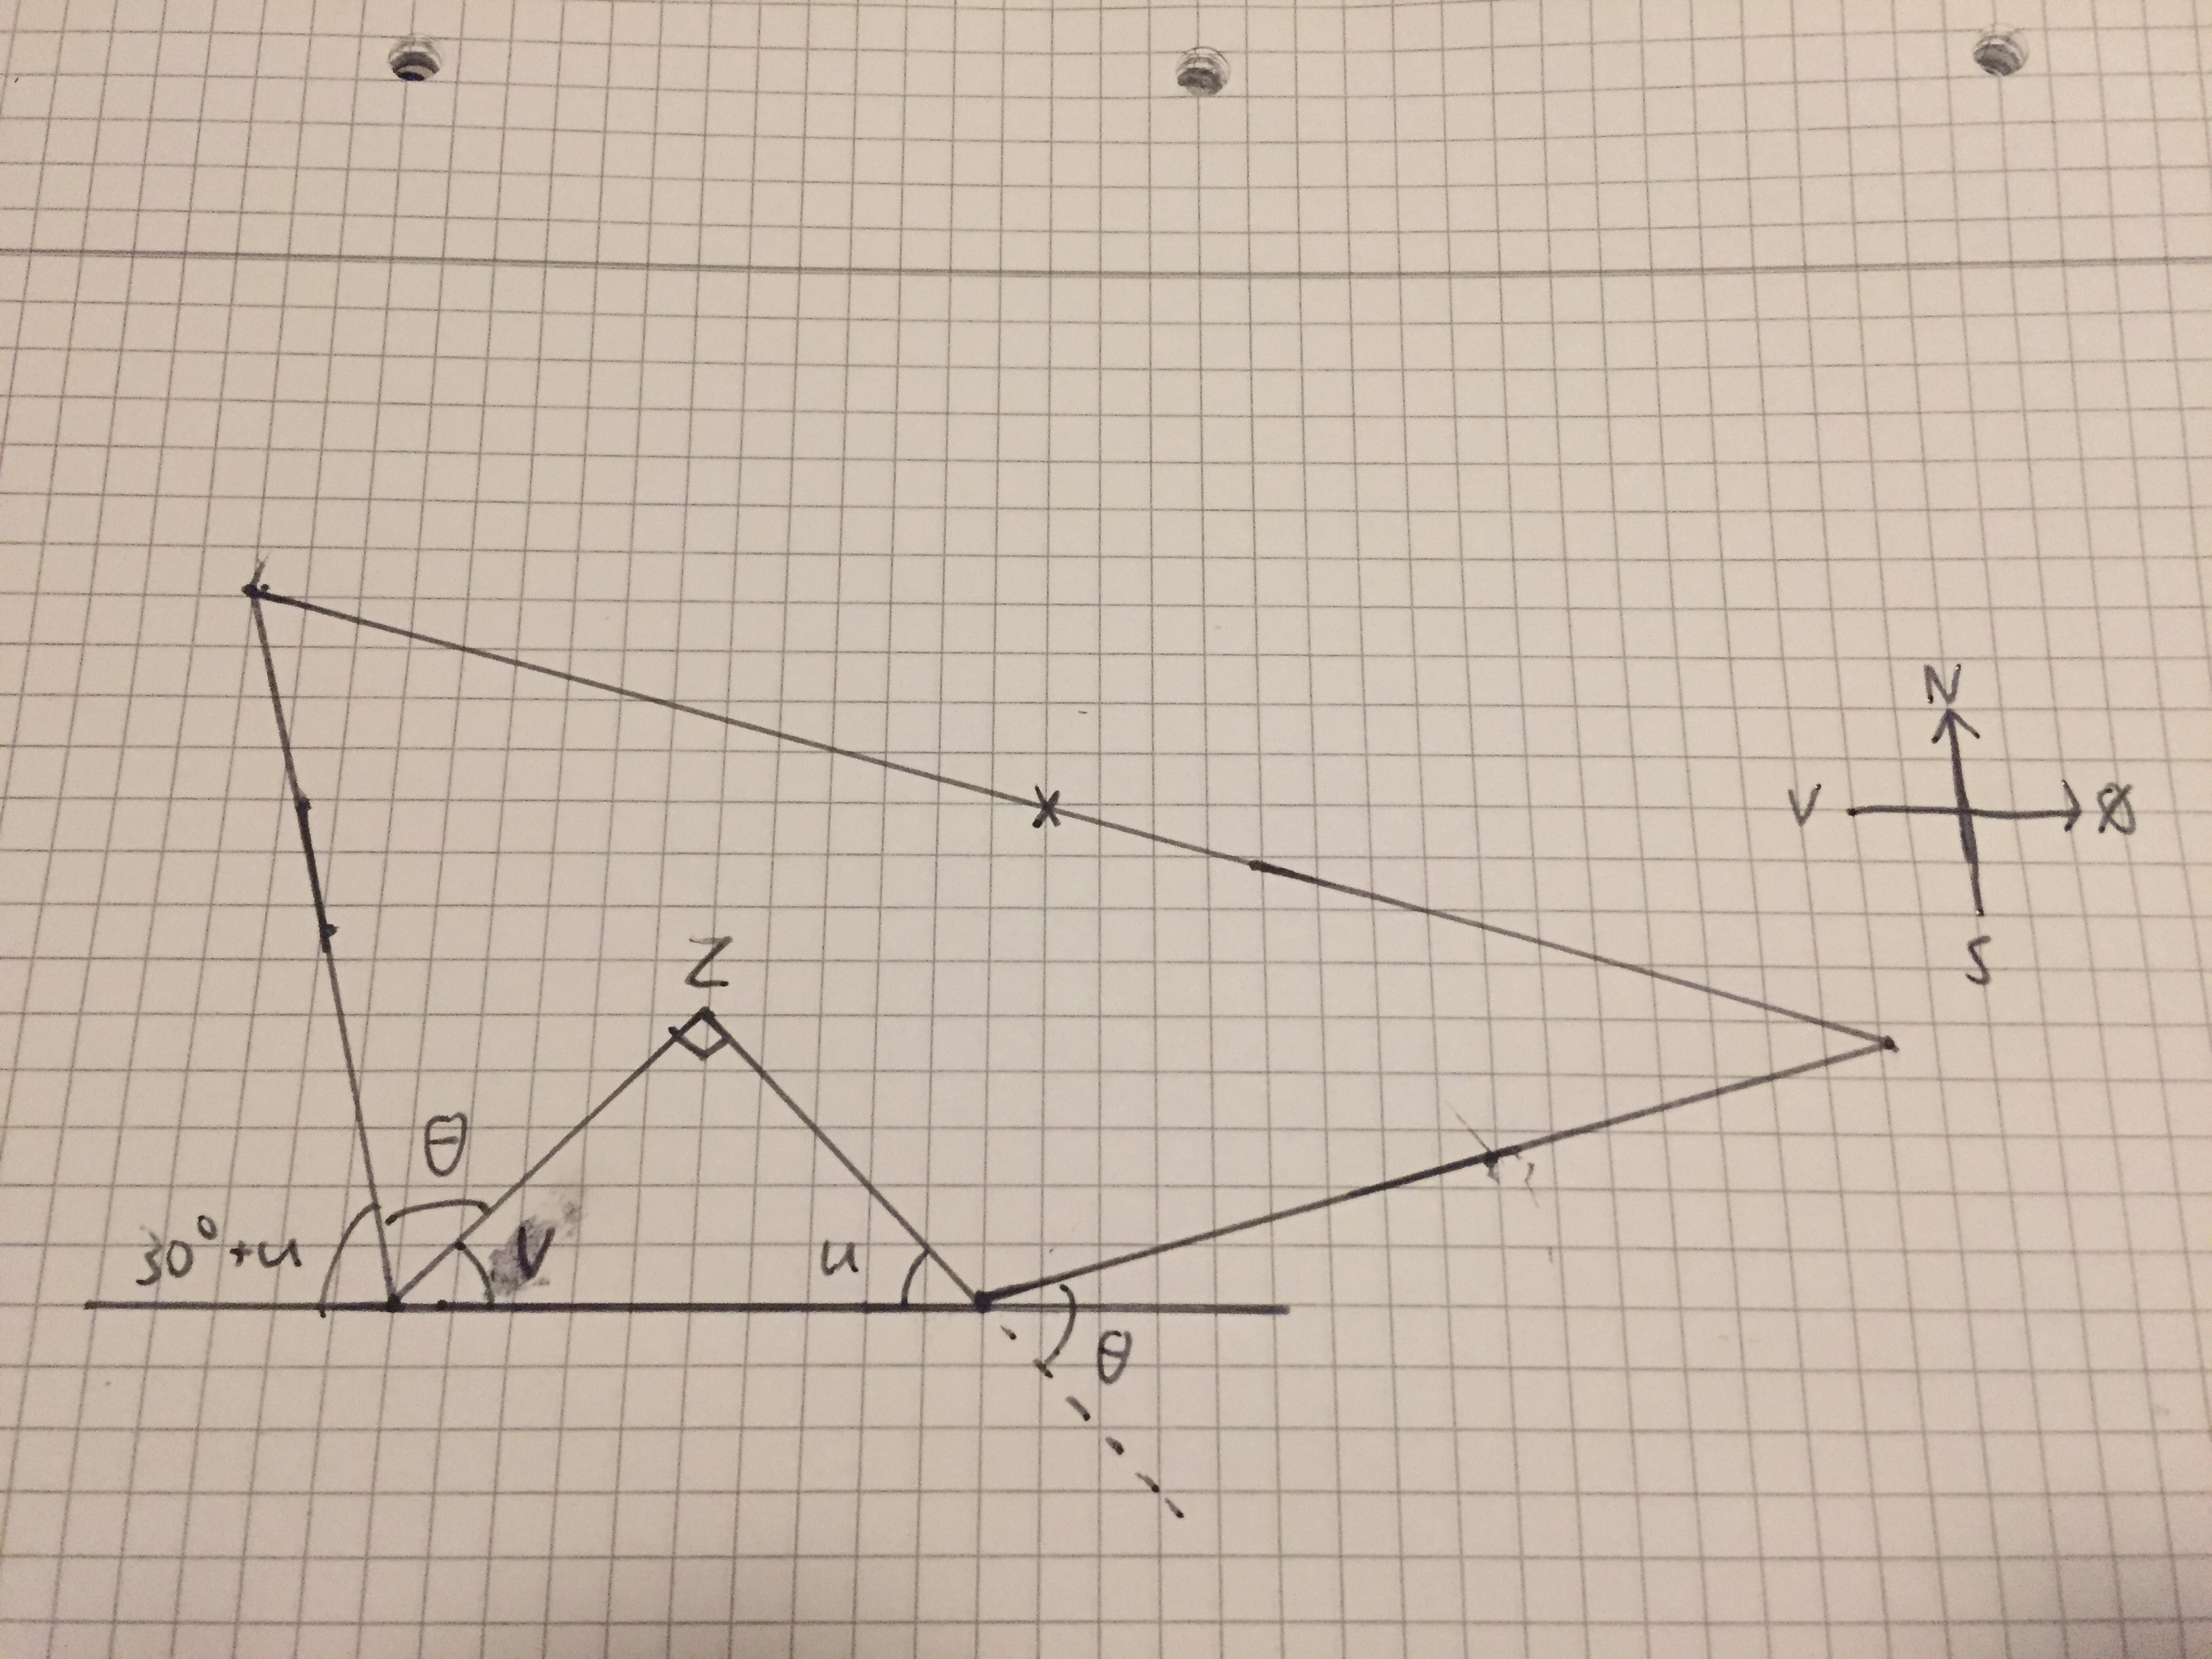
\includegraphics[scale=0.1]{pic_revised}
\\\\
Vi legger øya i det komplekse planet. Vi lar galgens posisjon være $Z$, og vi legger kordinatsystemet slik at 
vestlig palme ligger i origo og østlig palme ligger i punktet 1 på den reele aksen.
\\\\
a) Finn vinkel $\theta$ ved hjelp av tegningen over. \\\\

b) Vis at merket du skal sette etter at du har gått videre fra den vestlige palmen er i posisjon
$2e^{i\theta} \cdot Z$ og bruk vinkel $\theta$ som du fant for å lage et uttrykk for posisjonen. \\\\

c) Vis at merket du skal sette etter at du har gått videre fra den østlige palmen er i posisjon
$1 + 2e^{-i\theta} \cdot (1 - Z)$ og bruk vinkel $\theta$ som du fant for å lage et uttrykk for posisjonen. \\\\

d) Finn det komplekse tallet som tilsvarer skattens posisjon og vis hvordan man kan finne skatten uten å vite galgens posisjon. \\\\\\

\subsection*{Løsning:}
a) Vi ser at $(30^\circ + u) + \theta + v = 180^\circ$. For å finne $\theta$, så må man se at $v = 90^\circ - u$, og kan da sette opp ligningen:
\begin{equation}
    \begin{split}
        (30^\circ + u) + \theta + v &= 180^\circ \\
        (30^\circ + u) + \theta + (90^\circ - u) &= 180^\circ \\
        30^\circ + \cancel{u} + \theta + 90^\circ - \cancel{u} &= 180^\circ \\
        \theta + 120^\circ  &= 180^\circ \\
        \theta &= 60^\circ
    \end{split}
\end{equation}\\\\

b) Når man multipliserer et komplekst tall med $2e^{i\theta}$, så tilsvarer det en dreining på $\theta$ til venstre og en dobling av lengden. $Z$ tilsvarer da vektoren fra origo til $Z$. \\
Når man bruker $\theta = 60^\circ = \frac{\pi}{3}$, så vil man få et uttrykk:
\begin{equation}
    \begin{split}
        W_{\text{vest}} &= Z \cdot 2e^{i \cdot \frac{\pi}{3}} \\
                 &= Z \cdot 2 \cdot (\cos{\frac{\pi}{3}} + i\sin{\frac{\pi}{3}}) \\
                 &= Z \cdot 2 \cdot (\frac{1}{2} + \frac{\sqrt{3}}{2}i) \\
                 &= Z \cdot (1 + \sqrt{3}i) \\
                 &= Z + Z \cdot \sqrt{3}i
    \end{split}
\end{equation}

c) Når man multipliserer et komplekst tall med $2e^{i\theta}$, så tilsvarer det en dreining på $\theta$ til venstre og en dobling av lengden. $1 - Z$ tilsvarer da vektoren fra 1 til $Z$, og så legger man til $1$ i uttrykket fordi det er posisjonen til den østlige palmen. \\
Når man bruker $\theta = 60^\circ = \frac{\pi}{3}$, så vil man få et uttrykk:
\begin{equation}
    \begin{split}
        W_{\text{øst}} &= (1 - Z) \cdot 2e^{i \cdot \frac{\pi}{3}} \\
                &= 1 + (1 - Z) \cdot 2 \cdot (\cos{\frac{\pi}{3}} + i\sin{\frac{\pi}{3}}) \\
                &= 1 + (1 - Z) \cdot 2 \cdot (\frac{1}{2} + \frac{\sqrt{3}}{2}i) \\
                &= 1 + (1 - Z) \cdot (1 + \sqrt{3}i) \\
                &= 2 - Z + \sqrt{3}i - Z \cdot \sqrt{3}i
    \end{split}
\end{equation}

d) For å finne skattens posisjon så må man ta $\frac{W_{\text{vest}} + W_{\text{øst}}}{2}$. altså:
\begin{equation}
    \begin{split}
        s &= \frac{W_{\text{vest}} + W_{\text{øst}}}{2} \\
          &= \frac{(Z + Z \cdot \sqrt{3}i) + (2 - Z + \sqrt{3}i - Z \cdot \sqrt{3}i)}{2} \\
          &= \frac{\cancel{Z} + \cancel{Z \cdot \sqrt{3}i} + 2 - \cancel{Z} + \sqrt{3}i - \cancel{Z \cdot \sqrt{3}i}}{2} \\
          &= \frac{2 + \sqrt{3}i}{2} \\
          &= 1 + \frac{\sqrt{3}}{2}i
    \end{split}
\end{equation}
For å finne skatten, så må man gå fra den vestlige palmen til den østlige palmen og telle skrittene. Deretter så går man $\frac{\sqrt{3}}{2}$ av skrittene nord.



\newpage

\section*{Oppgave 4}
For å løse denne oppgaven, så har jeg valgt å finne den komplekse faktoriseringen først, og deretter gi
svarene for de ulike deloppgavene utifra denne faktoriseringen.
\newline\newline

\begin{flushleft}
Lar P være:
\begin{equation}
    P(z) = z^4 + z^3 + 25z^2 + 25z
\end{equation}
\newline

Ser at man kan faktorisere ut en $z$ og får:
\begin{equation}
    P(z) = z(z^3 + z^2 + 25z + 25)
\end{equation}
\newline

Vi kan også se at $(z + 1)$ er en faktor i polynomet ved å sette inn $z = -1$ i $P(z)$:
\begin{equation}
    \begin{split}
        P(-1) &= (-1)^4 + (-1)^3 + 25*(-1)^2 + 25*(-1) \\
              &= 1 + (-1) + 25 + (-25) \\
              &= 0
    \end{split}
\end{equation}
\newline

Da kan vi utføre polynomdivisjonen:
\begin{equation}
    \begin{split}
        &z^3 + z^2 + 25z + 25 : (z + 1) = z^2 + 25 \\
        \mathrlap{\underline{\phantom{-(z^3 + z^2)}}}-(&z^3 + z^2) \\
        &~~~~~~~0 \, + 25z + 25 \\
        &~~~~~~~~~ \mathrlap{\underline{-(25z + 25)}} \\
        &~~~~~~~~~~~~~~~~~~~~~~\,0
    \end{split}
\end{equation}
\newline

Deretter kan vi løse $z^2 + 25 = 0$ og får:
\begin{equation}
    \begin{split}
        z^2 + 25 &= 0 \\
        z^2 &= -25 \\
        z &= \pm \sqrt{-25} \\
        z &= \pm \sqrt{-1} \sqrt{25} \\
        z &= \pm 5i
    \end{split}
\end{equation}
\newline

Den komplekse faktoriseringen vil da bli:
\begin{equation}
    P(z) = z(z + 1)(z + 5i)(z - 5i)
\end{equation}
\newline\newline


    a) De komplekse røttene til P er $-5i$ \& $5i$. \\
    b) Den komplekse faktoriseringen til P er: $P(n) = z(z + 1)(z + 5i)(z - 5i)$ \\
    c) Den reele faktoriseringen til P er: $P(n) = z(z + 1)(z^2 + 25)$ 
\end{flushleft}
\newpage

\section*{Oppgave 5}
Først så finner man ut av hva følgen konvergerer mot hvis den konvergerer:
\begin{equation}
    \begin{split}
        \lim_{n \to \infty} a_{n+1} &= \lim_{n \to \infty} 2 + \frac{3}{4} a_n \\
        L &= 2 + \frac{3}{4} L \\
        \frac{1}{4} L &= 2\\
        L &= 8
    \end{split}
\end{equation}
Over, så byttet man ut $a_{n+1}$ og $a_n$ med $L$, og får at $L = 8$, som er hva følgen kan konvergere mot hvis den konvergerer. \\
For å bevise at $8$ er en oppad grense, så sjekker vi om $a_1 \leq 8$. \\
$a_1 = 0 \leq 8 $
Anta at $a_n \leq 8$. Da er:
\begin{equation}
    \begin{split}
        a_{n+1} = 2 + \frac{3}{4} a_n \leq 2 + \frac{3}{4} \cdot 8 = 2 + 6 = 8
    \end{split}
\end{equation}
Altså $a_{n+1} \leq 8$. Dermed er $a_n \leq 8$ for alle $n \geq 1$. \\ \\

Nå viser man at følgen er voksende, altså $a_{n+1} \geq a_n$ for alle $n \geq 1$
\begin{equation}
    a_{n+1} = 2 + \frac{3}{4}a_n
    \begin{split}
        2 + \frac{3}{4}a_n &\geq a_n \\
        2a_n + \frac{3}{4}a_n &\geq a_n \\
        \frac{8}{4}a_n + \frac{3}{4}a_n &\geq a_n \\
        \frac{11}{4}a_n &\geq a_n
    \end{split}
\end{equation}
Følgen er altså voksende.

\end{document}